\section{Évaluation du projet}

Dans cette partie, nous allons faire une évaluation du projet. Nous évaluerons d'abord le logiciel dans ses trois principales parties. Ensuite, nous verrons son utilisabilité pour les artistes et l'écriture de la chorégraphie. Enfin, d'une manière plus générale, nous aborderons la gestion du projet. 

\subsection{Validation du logiciel} %validation des fonctionnalités du logiciel 

Dans cette partie, nous vérifions que les principales fonctionnalités sont correctes. On s'intéressera aux trois parties du logiciel séparemment: la visualisation, la communication et la simulation. 

\subsubsection{Visualisation}

Concernant la visualisation, les trois critères importants pour évaluer cette partie sont : la fluidité des mouvements, la maniabilité de l'environnement 3D et l'ergonomie de l'interface utilisateur. 

La fluidité des images est assurée par un nombre d'images par seconde (fps) fixé à 60, ce qui permet d'avoir un rendu agréable et fluide. La chorégraphie imaginée par les étudiants compterait 10 robots Metabot, et pour ce nombre le nombre d'images par seconde est toujours 60 fps : l'image est fluide et l'interface réagit instanément (pour un utilisateur, la différence de vitesse ne se sent pas entre 1 et 10 robots).
Nous avons testé pour 100 robots, le lancement de l'application prend du temps et le nombre d'images par seconde est divisé par 2, on a donc 30 fps ce qui reste correct pour une visualisation. 

La maniabilité de l'environnement 3D repose principalement sur les déplacements de la camera de type rotation et zoom. Les deux sont rendus possibles grâce à la classe \verb|EasyCam| d'openFrameworks qui permet d'avoir une camera simple munie des fonctionnalités usuelles (rotation, zoom, calibrage à l'initialisation automatique par rapport au milieu de la scène). Ainsi, l'utilisateur retrouve un environnement 3D usuel.

Nous avons essayé de penser à l'ergonomie, en rajoutant des menus déroulant pour chaque robot dans l'interface, ce qui permet d'éviter que le panel n'envahisse tout l'écran. De plus, un message d'aide est affiché au lancement du logiciel, il explique les touches à appuyer pour afficher des axes ou la graduation en plus, et aussi pour cacher ce message d'aide.
De même l'affichage de message de sélection permet à l'utilisateur d'identifier facilement les robots,  ans qu'il ait à regarder le panel des positions.

Par ailleurs, pour alerter l'utilisateur de collision, nous avons choisi d'afficher un cercle rouge à l'emplacement du cercle mais aussi d'afficher un message de warning en haut de l'écran. Cela permet d'assurer que cet événement soit bien visible. En effet, si l'utilisateur zoom sur d'autres robots, il risque de ne pas voir le cercle rouge, alors que le message est toujours affiché au même endroit puisqu'il ne dépend pas de la scène 3D. Le cercle rouge permet tout comme le message de sélection, d'identifier plus facilement l'emplacement de la collision.

\subsubsection{Communication réseau}

Au niveau de la communication, nous avons comparé la fréquence d'appel à la méthode \verb|update| de la classe \verb|ofApp| de mise à jour de la scène par rapport à la fréquence d'i-score. En effet, on pourrait avoir des problèmes de temps si la méthode \verb|update| était appelée à une fréquence moins élevée que le tic d'i-score car on pourrait avoir des données d'i-score qui ne seraient pas utilisées par simulationRainOfmusic (si par exemple \verb|update| est appelée toutes les 5s et que le tic d'i-score est de 2s). 

En réalité, la méthode \verb|update| est appelée toute les 16 ms et le tic d'i-score est de 40 ms par défaut. Ainsi, les données utilisées par simulationRainOfMusic sont toujours synchronisées par rapport à celles d'i-score. On pourrait même imaginer une petite diminution de la fréquence d'appel à \verb|update| pour soulager l'utilisation de ressources, notamment lors d'une représentation avec beaucoup de robots. 

\subsubsection{Simulation}

A propos du côté simulation du logiciel, plusieurs aspects peuvent être vérifiés.

D'abord, l'échelle spatio-temporelle : chaque graduation représente un mètre et si on choisit $dx=100 mm.s^{-1}$ ou $dy=100 mm.s^{-1}$ pour un metabot, celui-ci avance bien d'une graduation toutes les dix secondes.

Ensuite, on peut s'intéresser à la batterie des robots. Celle-ci se décrémente bien linéairement en fonction de la distance parcourue par le robot en question. A l'arrêt, les robots ne consomment pas puis si on fait parcourir dix mètres à un robot, on peut voir que la même quantité de batterie est consommée sur chaque mètre. Des expérimentations pourraient être faites pour avoir un modèle de consommation plus réaliste. Par exemple, on pourrait s'intéresser à la consommation à l'arrêt ou selon la vitesse et la fréquence de pas quand le metabot est en mouvement.

Enfin, pour la perte de paquet, on peut compter le nombre de paquets perdus et reçus et retrouver le pourcentage de perte correspondant. Pour que celui-ci soit réaliste, on pourrait faire des expérimentations pour l'évaluer mais le protocole de communication n'est pas encore décidé définitivement (bluetooth ou XBee). 

\subsection{Confrontation du logiciel avec les artistes}

Dans le cadre d'une rencontre avec les artistes, nous avons pu commencer à écrire la chorégraphie qu'ils avaient conçu. Celle-ci est présentée dans la figure suivante \ref{chore}:



%\hspace*{-12cm}
\begin{figure}
\centering
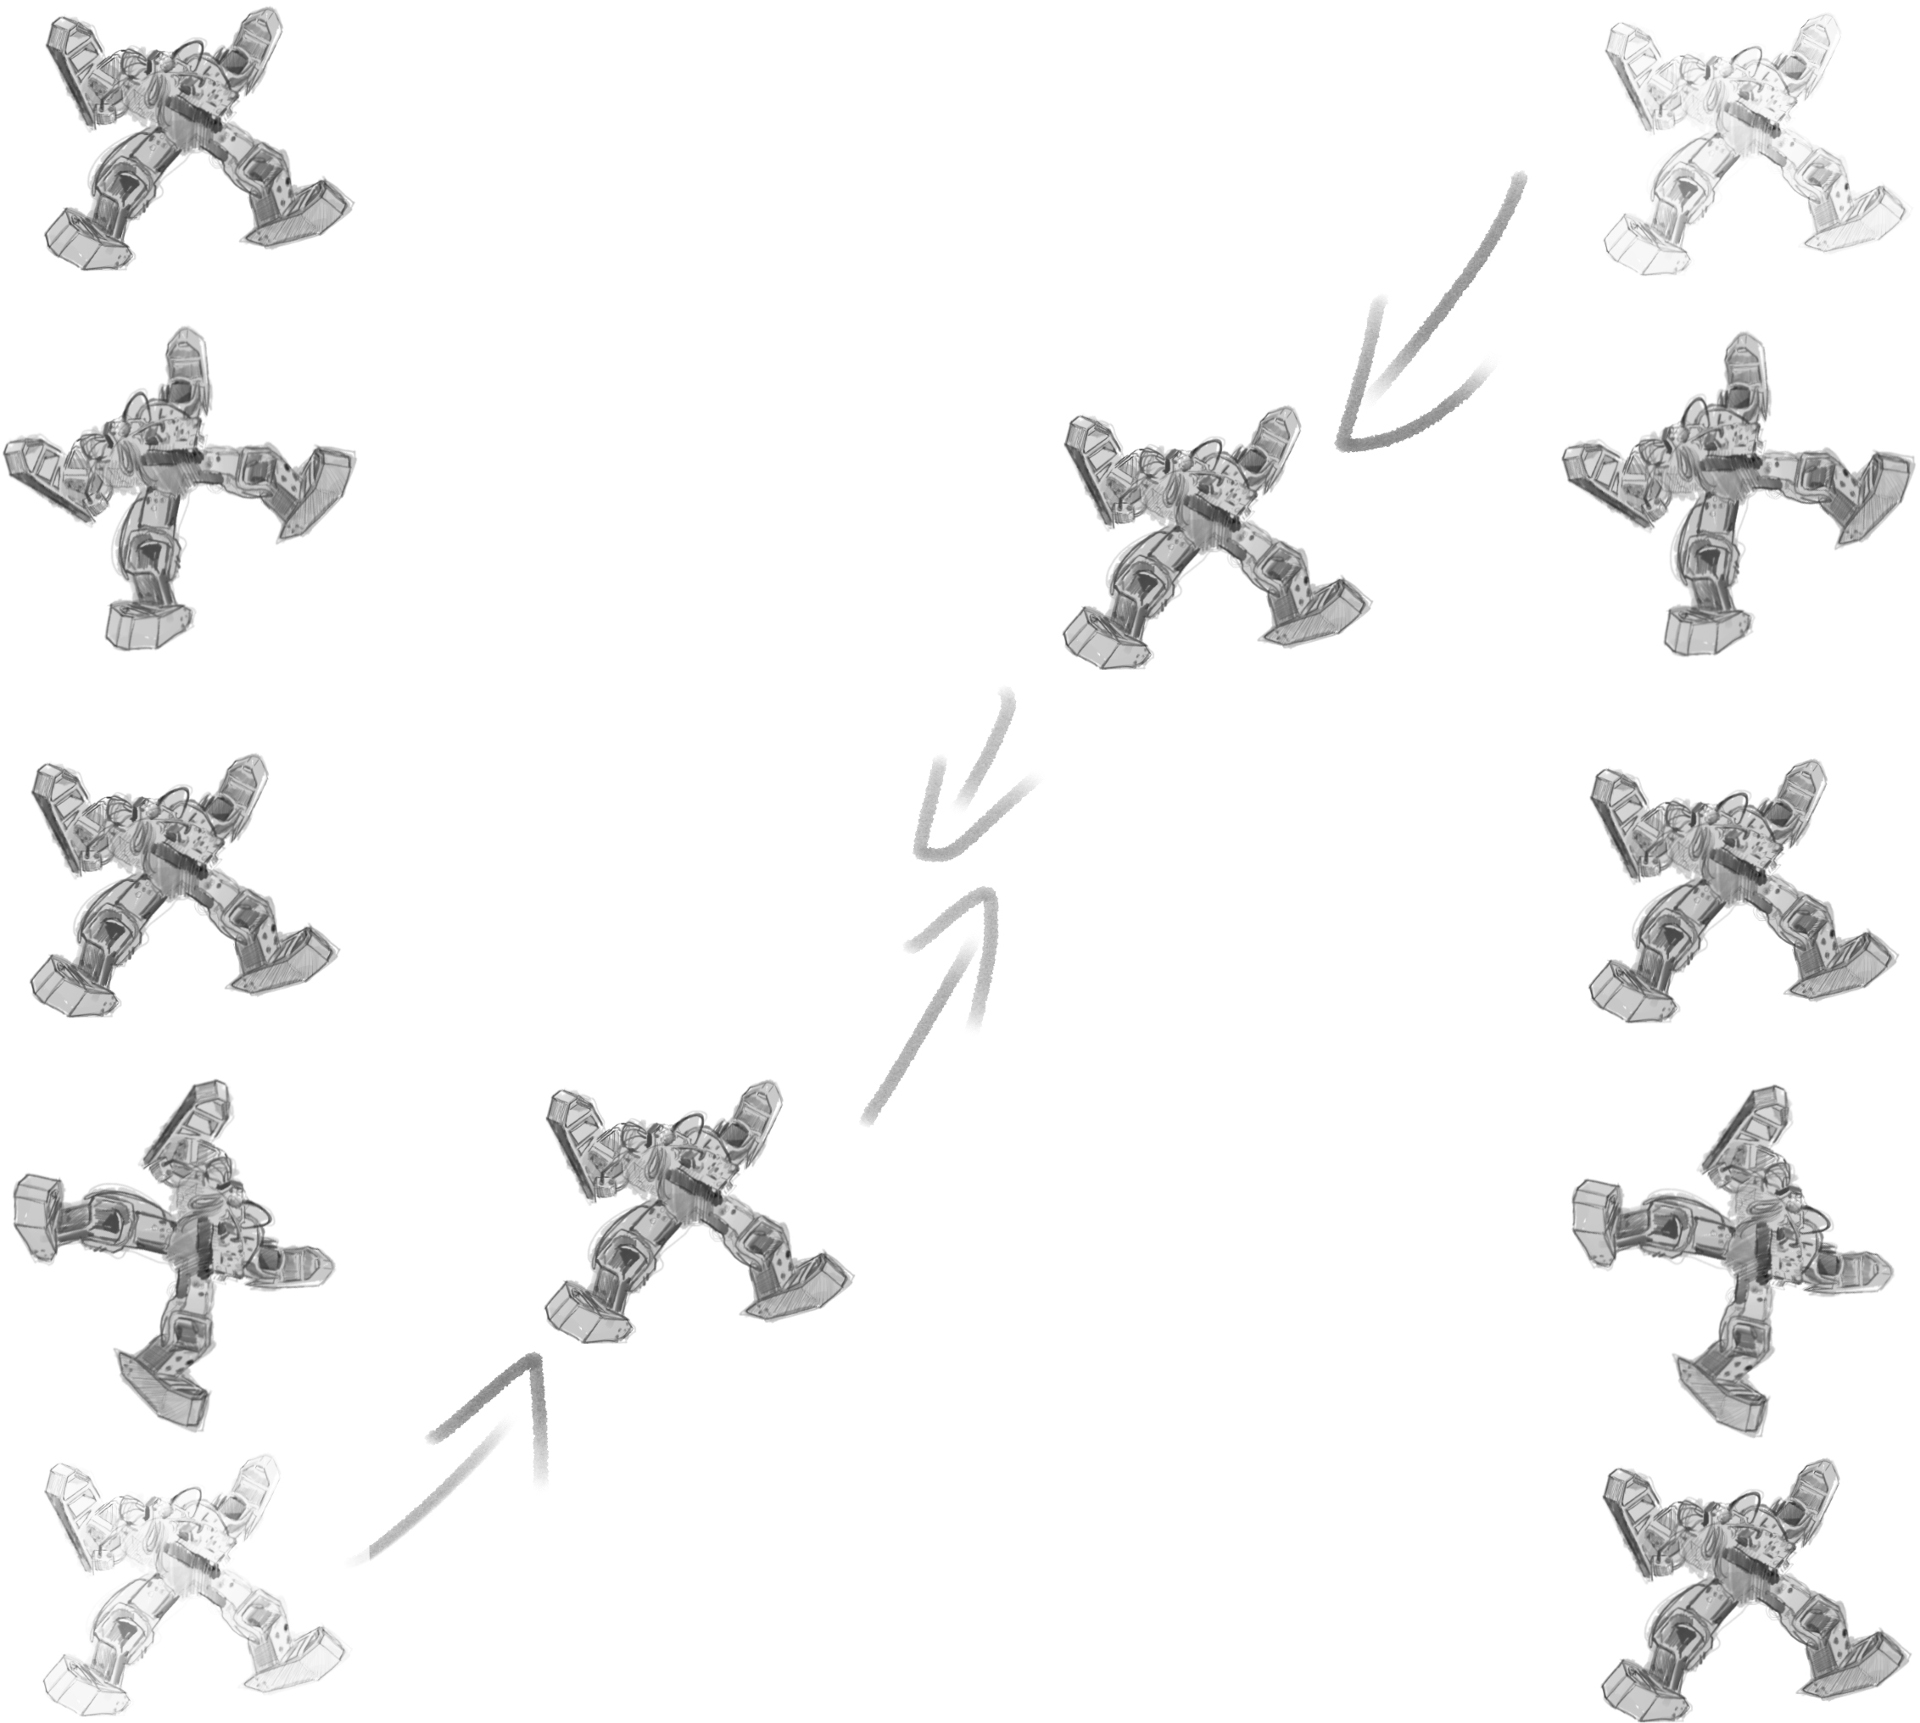
\includegraphics[scale=0.5]{reveildessin}
\caption{Dessin original des étudiants d'art de Bilbao}
\label{chore}
\end{figure}


\begin{figure} %[htbp]
\centering
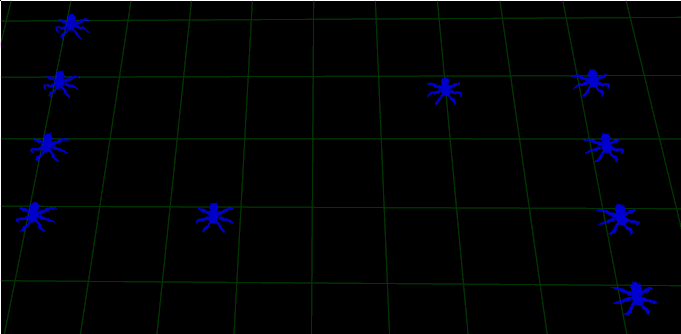
\includegraphics[scale=0.8]{reveil2}
\caption{Simulation du tableau avec notre interface simulationRainOfMusic}
\label{reveil}

\end{figure}

- mettre l'image de la chorégraphie

Dans cette chorégraphie, il faudra notamment que les metabots décrivent un cercle. Ceci a déjà pu être fait dans simulationRainOfMusic.

- pas eu le temps de tester une chorégraphie conçue avec notre logiciel sur un robot.


\subsection{Gestion du projet: calendrier et difficultés}

Dans cette partie, nous verrons la gestion du projet par rapport au calendrier que nous nous étions fixé. Puis nous verrons les difficultés que nous avons rencontrées. Un calendrier bilan est représenté sur la figure suivante \ref{cal}:

\begin{figure}[H]
  \begin{center}
  	\includegraphics[scale=0.7]{imgs/calendrierbis.png}
  	\caption{Calendrier bilan. En noir ce qui était prévu. En rouge ce qui était prévu mais qui n'a pas été fait. En vert ce qui a été fait mais qui n'était pas prévu}
  	\label{cal}
  \end{center}
\end{figure}

On remarque que finalement le calendrier de départ a subi beaucoup de changements. D'une part, la partie de simulation des mouvements des drones a été abandonnée car le projet s'est focalisé sur la mise en place des métabots en premier. D'autre part, la partie communication ne s'est pas déroulée comme prévu. L'intégration de la communication avec i-score dans simulationRainOfMusic (intégration de l'API d'OSSIA dans simulationRainOfMusic) nous a pris du temps. Une fois l'API en place, la communication avec i-score se fait assez facilement. 

Ensuite, l'ajout des panels dans l'interface de simulationRainOfMusic et la possibilité de modifier les paramètres des robots via ces panels a posé deux problèmes: la communication entre l'interface et le reste du logiciel, qui a donné lieu à la classe \verb|Parameter| et la synchronisation entre l'interface de simulationRainOfMusic et i-score. En effet, pour ce dernier, une boucle infinie peut facilement apparaître comme vu précédemment car les listener vers i-score et vers l'interface de simulationRainOfMusic déclenchent automatiquement la mise à jour des valeurs qu'ils écoutent. 

